\documentclass[30pt,twocolumn,letterpaper]{article}
\usepackage{cvpr}
\usepackage{times}
\usepackage{booktabs}
\usepackage{epsfig}
\usepackage{graphicx}
\usepackage{amsmath}
\usepackage{amssymb}
\cvprfinalcopy
\def\cvprPaperID{****}
\def\httilde{\mbox{\tt\raisebox{-.5ex}{\symbol{126}}}}
\usepackage{graphicx}
\usepackage{indentfirst}
\setlength{\parindent}{2em}
\usepackage{cite}
\usepackage[colorlinks,linkcolor=red,anchorcolor=blue,citecolor=green,backref=page]{hyperref}
\author{Qilei Zhang}
\date{May 31 2018}
\title{Quantum stochastic resonance}
\begin{document}
\maketitle
\begin{abstract}
   Recently, the question has been posed whether stochastic resonance manifests itself on a quantum scale. In particular, recent experiments in a macroscopic quantum system, such as a superconducting quantum interference device, established the mechanism of stochastic resonance in the classical regime of thermal activation.
\end{abstract}
\section{Introduction}
The experimental work of Rouse, Han, and Lukens also addressed nonlinear stochastic resonance, such as the noise-induced resonances, which are elucidated in Sec. VII.D.1 below\cite{Kim2006Stochastic}.
\begin{figure}[htbp]
\small
\centering
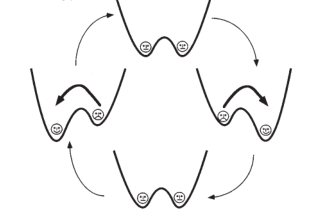
\includegraphics[width=20em]{000.png}
\caption{23 Bistable ring laser}
\label{fig:lable}
\end{figure}
\section{Quantum corrections to stochastic resonance}
Let us first focus on the regime T>=T0 , where quantum tunneling is not the dominant escape path, but nevertheless leads to significant quantum corrections. The role of quantum tunneling in this regime has been investigated only recently by Grifoni et al. These authors investigated the dissipative inertial bistable quantum dynamics x(t) at thermal temperature T in a double-well configuration which is modulated by the periodic force A0 cos(Vt)\cite{Kurt2002Stochastic}. \\
\begin{equation}
r_n=\frac{1}{T}\int_0^T r(t)exp(-inwt)dt
\end{equation}
\begin{table}
\begin{center}
\begin{tabular}{cccccccc}
\toprule
         & 1 &  2  &   3  &  4  &  5  &  6  & 7 \\
\midrule
Alphabet & A &  B  &   C  &  D  &  E  &  F  & G\\
Roman    & I &  II &  III &  IV &  V  &  VI & VII\\
\bottomrule
\end{tabular}
\end{center}
\caption{Results.   Ours is better.}
\end{table}
\section{Quantum stochastic resonance in the deep cold}
The situation changes drastically when we proceed towards the extreme cold. Here, we shall focus on the deep quantum regime, where tunneling is the only channel for barrier crossing. In this low-temperature regime, periodic driving induces several new interesting, counterintuitive physical phenomena, such as coherent destruction of tunneling, the stabilization of dissipative coherence with increasing temperature\cite{Wellens2004Stochastic}.
{\small
\bibliographystyle{ieee}
\bibliography{1}
}
\end{document}
